\setchapterstyle{kao}
\setchapterpreamble[u]{\margintoc}

\chapter{Search for an Excess of Heavy Neutral Lepton Events}
\labch{analysis}

The measurement performed in this thesis is the search for an excess of HNL events in the \SI{10}{years} of IceCube DeepCore data. In principle the two physics parameters to be probed are the mass of the HNL, $m_4$, and the mixing between the fourth heavy mass state and the SM $\tau$ sector, $|U_{\tau4}|^2$. Since the mass itself influences the production and decay kinematics of the event and the accessible decay modes, individual mass sets were produced as described in \refsec{model_specific_simulation}. The mass slightly influences the energy distribution, while the mixing both changes the overall scale of the HNL events and the shape in energy and PID. IceCube DeepCore is suited to measure the excess which appears around and below \SI{20}{\gev}, due to its production from the atmospheric tau neutrinos, although a reduced lower energy threshold could improve the analysis. The measurement will be performed for the three mass sets individually, while the mixing is the parameter that can be varied continuously and will be measured in the fit. 


\section{Final Level Sample} \labsec{analysis_samples}

The final level sample of this analysis always consists of the neutrino and muon MC introduced in \refsec{sm_event_generation} and one of the three HNL samples explained in \refsec{model_specific_simulation}. All of those simulation sets and the \SI{10}{years} of IceCube DeepCore data are processed through the full processing and event selection chain described in \refsec{processing_chain} and \refsec{reconstruction} leading to the final level sample. Since applying the last cuts from \refsec{analysis_cuts} leaves an insignificant amount of pure noise events in the sample, the noise simulation is not included in the analysis and will not be listed here.


\todo{add information about the matter profile used }
\todo{add information about the oscillation probability calculation and the software used for it}

\subsection{Expected Rates/Events}

The rates and the expected number of events for the SM background are shown in \reftab{background_final_level_expectation}. The explicit detector livetime in the \SI{10}{} years data taking period is \SI{9.28}{years}. The rates are calculated by summing the weights of all events in the final level sample, while the uncertainties are calculated by taking the square root of the sum of the weights squared. The expected number of events is calculated by multiplying the rate with the livetime. The individual fractions show that this sample is neutrino dominated where the majority of events are $\nu_\mu$-CC events.

\begin{table}[h]
    \begin{tabular}{ lccc }
    \hline\hline
    \textbf{Type} & \textbf{Rate [\si{\milli\hertz}]} & \textbf{Events (in \SI{9.28}{years})} & \textbf{Fraction [\si{\percent}]} \\ 
    \hline\hline
    $\nu_\mu^\rm{CC}$   & 0.3531 & 103321 $\pm$ 113 & 58.9 \\
    $\nu_e^\rm{CC}$     & 0.1418 & 41490 $\pm$ 69 & 23.7 \\
    $\nu_\rm{NC}$       & 0.0666 & 19491 $\pm$ 47 & 11.1 \\
    $\nu_\tau^\rm{CC}$  & 0.0345 & 10094 $\pm$ 22 & 5.8 \\
    $\mu$               & 0.0032 & 936 $\pm$ 15 & 0.5 \\
    \hline
    total               & 0.5991 & 175336 $\pm$ 143 & 100.0  \\
    \hline
    \end{tabular}
\caption[Final level background event/rate expectation]{Final level rates and event expectation of the SM background particle types.}
\labtab{background_final_level_expectation}
\end{table}

\todo{Should I adapt the total numbers to match the sum of the rounded individual parts?}

\reftab{signal_final_level_expectation} shows the rates and expected number of events for the HNL signal simulation. The expectation depends on the mass and the mixing and shown here are two example mixings for all the three masses that are being tested in this work. A mixing of $0.0$ would result in no HNL events at all. It can already be seen that for the smaller mixing of $|U_{\tau4}|^2=10^{-3}$ the expected number of events is very low, while at the larger mixing of $|U_{\tau4}|^2=10^{-1}$ the number is comparable to the amount of muons in the background sample. 

\begin{table}[h]
    \begin{tabular}{ lcc }
    \hline\hline

    \textbf{HNL mass} & \textbf{Rate [\si{\micro\hertz}]} & \textbf{Events (in \SI{9.28}{years})} \\

    \hline\hline
    \textbf{$|U_{\tau4}|^2=10^{-1}$} & & \\ 
    \hline
    \SI{0.3}{\gev} & 3.3298 $\pm$ 0.0053 & 974.5 $\pm$ 1.6 \\
    \SI{0.6}{\gev} & 3.0583 $\pm$ 0.0058 & 895.0 $\pm$ 1.7 \\
    \SI{1.0}{\gev} & 2.4988 $\pm$ 0.0059 & 731.3 $\pm$ 1.7 \\
    \hline
    \textbf{$|U_{\tau4}|^2=10^{-3}$} & & \\ 
    \hline
    \SI{0.3}{\gev} & 0.0057 & 1.67 $\pm$ 0.01 \\
    \SI{0.6}{\gev} & 0.0220 & 6.44 $\pm$ 0.01 \\
    \SI{1.0}{\gev} & 0.0248 & 7.27 $\pm$ 0.01 \\
    % \SI{0.3}{\gev} & 0.00571 $\pm$ 0.00002 & 1.67 $\pm$ 0.01 \\
    % \SI{0.6}{\gev} & 0.02200 $\pm$ 0.00004 & 6.44 $\pm$ 0.01 \\
    % \SI{1.0}{\gev} & 0.02484 $\pm$ 0.00005 & 7.27 $\pm$ 0.01 \\
    \hline
    \end{tabular}
\caption[Final level signal event/rate expectation]{Final level rates and event expectations of the HNL signal for all three masses and two example mixing values.}
\labtab{signal_final_level_expectation}
\end{table}


\subsection{Analysis Binning}

The identical binning to the analysis performed in \sidecite{flercnn_analysis_result} is used. It was chosen such that the track-like bin has the largest $\nu_\mu$-CC fraction. Extend the binning towards lower energies or increasing the number of bins did not improve the HNL sensitivities significantly. It also has to be considered that sufficient data events need to end up in the individual bins to result in a good fit, which was already investigated in the previous analysis. To mitigate the low data statistics, a few bins were not taken into account in the analysis. There are three bins in PID (cascade-like, mixed and track-like), 12 bins in reconstructed energy, and 8 bins in cosine of the reconstructed zenith angle as specified in \reftab{analysis_binning}. Originally, there were two more bins in $\cos(\theta)$, which were removed to reduce muons coming from the horizon and some low energy bins in the cascade-like bin are removed due to the low event statistics.
\begin{table}[h]
        \begin{tabular}{ llll }
        \hline\hline    
        \textbf{Variable} & \textbf{$N_\rm{bins}$} & \textbf{Edges} & \textbf{Step} \\     
        \hline\hline    
        $P_\nu$ & 3 & [0.00, 0.25, 0.55, 1.00] & linear \\
        $E$ & 12 & [5.00, 100.00] & logarithmic \\
        $\cos(\theta)$ & 8 & [-1.00, 0.04] & linear \\    
        \hline
        \end{tabular}
    \caption[Analysis binning]{Three dimensional binning used in the analysis. All variables are from the FLERCNN reconstruction explained in \refsec{reconstruction}.}
    \labtab{analysis_binning}
\end{table}

\todo{add 3D expectation and/or S/sqrt(B) plots}
\todo{Add fractions of the different particle types in the bins for benchmark mass/mixing (another table?)}


\section{Statistical Analysis} \labsec{analysis_principle}


\subsection{Low Energy Analysis Framework} \labsec{analysis_framework}

The analysis is performed using the \textsc{PISA} \sidecite{pisa_paper} \cite{pisa_software} software framework, which was developed to perform analyses "of small signals in high-statistics neutrino oscillation experiments". It is used to generate the expected event distributions from several MC sets, which can then be compared to the observed data. The expectation for each set is calculated in parallel, applying physics and nuisance parameter effects in a stage-wise manner, before combining the final expectation from all the sets.


\subsection{Test Statistic}

\todo{I feel like I have to be a bit more precise on what is the fit metric (e.g. the mod chi2) and what is the TS, as in the mod chi2 difference, which is the actual TS, right?}

The measurements are performed by comparing the weighted MC to the data. Through variation of the nuisance and physics parameters that govern the weights, the best matching set of parameters can be found. The comparison is done using a modified $\chi^2$ defined as
\begin{equation}
    \chi^2_{\mathrm{mod}} = 
    \sum_{i \in \mathrm{bins}}^{}\frac{(N^{\rm{exp}}_i - N^{\mathrm{obs}}_i)^2}
    {N^{\rm{exp}}_i + (\sigma^{\mathrm{\nu}}_i)^2 + (\sigma^{\mathrm{\mu}}_i)^2 + (\sigma^{\mathrm{HNL}}_i)^2}
     + \sum_{j \in \mathrm{syst}}^{}\frac{(s_j - \hat{s_j})^2}{\sigma^2_{s_j}}
    \;,
    \labeq{mod-chi2-hnl}
\end{equation}
as the \textit{test statistic (TS)}. The total even expectation is $N^{\rm{exp}}_i = N^{\mathrm{\nu}}_i + N^{\mathrm{\mu}}_i + N^{\mathrm{HNL}}_i$, where $N^{\mathrm{\nu}}_i$, $N^{\mathrm{\mu}}_i$, and $N^{\mathrm{HNL}}_i$ are the expected number of events in bin $i$ from neutrinos, atmospheric muons, and HNLs, while $N^{\mathrm{obs}}_i$ is the observed number of events in bin $i$. The expected number of events from each particle type is calculated by summing the weights of all events in the bin $N^{\mathrm{type}}_i = \sum_i^\rm{type}\omega_i$, with the statistical uncertainty being $(\sigma^{\mathrm{type}}_i)^2 = \sum_i^\rm{type}\omega_i^2$. The additional term in \refeq{mod-chi2-hnl} is included to apply a penalty term for prior knowledge of the systematic uncertainties of the parameters where they are known. $s_j$ are the systematic parameters that are varied in the fit, while $\hat{s_j}$ are their nominal values and $\sigma_{s_j}$ are the known uncertainties.

\todo{Do I want/need to include the description of the KDE muon estimation?}


\subsection{Physics Parameters} \labsec{analysis_parameters}

The only variable physics parameter in this analysis is the mixing between the HNL and the SM $\tau$ sector, $|U_{\tau4}|^2$. It can be changed continuously in the range of [\SI{0.0}, \SI{1.0}] by applying the weighting scheme described in \refsec{hnl_weighting_scheme}. The fit is initialized at the nominal value of \SI{0.0}. The other physics parameter, the mass $m_4$ of the HNL, is fixed to one of the three discrete masses to be tested, by using the corresponding sample of the HNL simulation described in \refsec{model_specific_simulation}.


\subsection{Nuisance Parameters} \labsec{analysis_systematics}

\begin{marginfigure}
    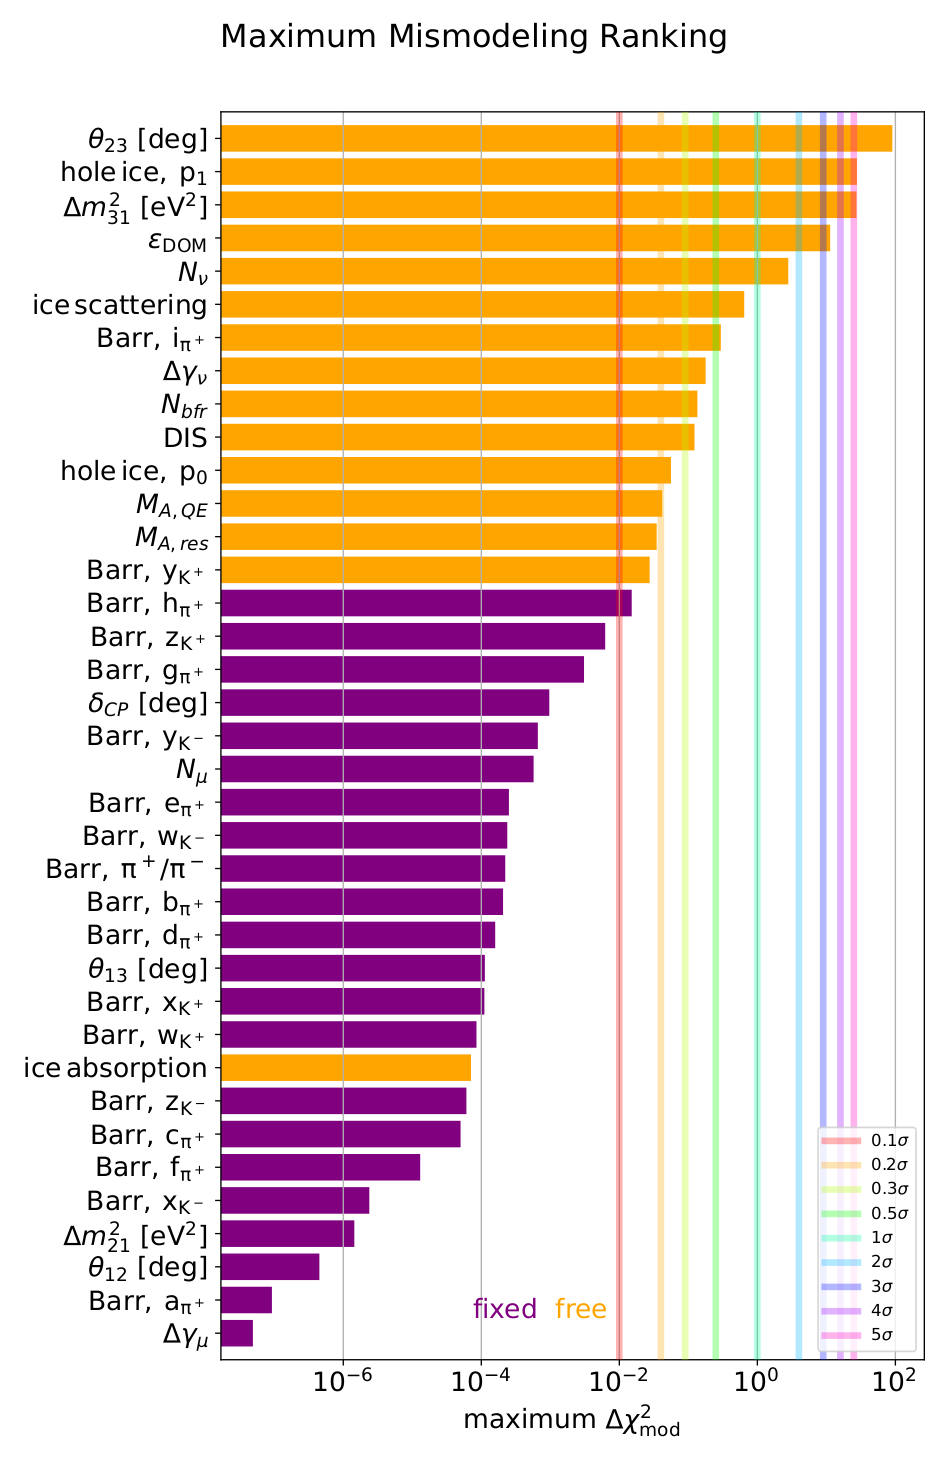
\includegraphics{figures/results/checks/plot_systematic_impact_ranking.png}
	\caption[xx]{"calculated at a mixing of 0.1 and for the 1.0 GeV set"}
    \labfig{systematic_impact_test}
\end{marginfigure}
\todo{Blow up labels/legend/title and make it more readable in the margin}
To decide which systematic uncertainties should be included in the fit, we test the potential impact they have on the TS if they are neglected. The test is performed by creating Asimov data using the \SI{1.0}{\gev} sample at a mixing value of \SI{0.0}, which is around the value where the analysis starts to become sensitive. The systematic parameter of interest is set to a value above its nominal expectation, either pulled up by $+1\sigma$ or by an educated estimate for parameters without a well-defined uncertainty. A fit is performed fixing the systematic parameter of interesting and leaving all additional parameters free. The resulting TS is the mis-modeling significance between a fit with all parameters free, which would result in a TS of 0.0 for this Asimov test\todo{I don't like this formulation, but don't know better right now..}. Parameters below a significance of \SI{0.1}{\sigma} are fixed and the test is perfomed in an iterative manner until the final set of free parameters is found. \reffig{systematic_impact_test} shows the resulting significances of one of these tests. In the final selection of free parameters the Barr $h_{\pi^+}$ parameter was also left free\todo{elaborate why this is also done to cover the whole energy range for the pion production, referencing the Barr Block plot that I haven't included yet :D} and the ice absorption is kept free, despite showing a small significance. This is done because the bulk ice parameters are not well constrained and are known to have large impact, which might be concealed in the test, due to correlations with the other parameters\todo{I truly dislike this sentence, too, better ideas?}.

\todo{I'm just writing out the data from the table, but I need to mention/motivate the included priors here and maybe just point to the table for the ranges/nominal values? (Not quite sure about this)}The scaling parameter $N_{\nu}$ is included to account for the unknown overall normalization of the neutrino rate. It has the identical effect on the SM neutrino events and the BSM HNL events and its nominal value is set to 1.0 with a wide range of [\SI{0.1}, \SI{2.0}].

Concerning the atmospheric neutrino flux, the CR power law flux correction factor $\Delta \gamma_\nu$ is included with nominal value of \SI{0.0} and a range of [\SI{-0.5}, \SI{0.5}]. Additionally, the Barr $h_{\pi^+}$, Barr $i_{\pi^+}$, and Barr $y_{K^+}$ parameters of the pion and kaon production uncertainties are included with nominal values of \SI{0.0} and ranges of [\SI{-0.75}, \SI{0.75}], [\SI{-3.05}, \SI{3.05}], and [\SI{-1.5}, \SI{1.5}], respectively.

From the cross-section uncertainties introduced in \refsec{cross_section_uncertainties}, all three parameters $\rm{DIS}$, $M_\rm{A,QE}$, and $M_\rm{A,res}$ are included in the fit with nominal values of \SI{0.0} for all of them and range [\SI{-0.5}, \SI{1.5}] for $\rm{DIS}$ and [\SI{-2.0}, \si{2.0}] for the axial mass parameters $M_\rm{A,QE}$, and $M_\rm{A,res}$.

All the detector systematic uncertainties are included in the fit. The DOM efficiency $\epsilon_{\rm{DOM}}$ has a nominal value of \SI{1.0} and a range of [\SI{0.8}, \SI{1.2}]. It is constrained by a Gaussian prior with a width of \SI{0.1}. The hole ice model parameters $p_0$ and $p_1$ are included with nominal values of \SI{0.101569} and \SI{-0.049344}, respectively, and ranges of [\SI{-0.6}, \SI{0.5}] and [\SI{-0.2}, \SI{0.2}]. The bulk ice absorption and scattering parameters are included with nominal values of \SI{1.0} and \SI{1.05}, respectively, and ranges of [\SI{0.85}, \SI{1.15}] and [\SI{0.9}, \SI{1.2}]. They are unconstrained in the fit and the ranges are set to be conservative determined from calibration data\todo{cite?!}

The two atmospheric neutrino oscillation parameters $\theta_{23}$ and $\Delta m^{2}_{31}$ are also included in the fit with nominal values of \SI{47.5047}{\degree} and \SI{2.475e-3}{\electronvolt^2}, respectively. Since they govern the shape and the strength of the tau neutrino flux, by defining the oscillation from $\nu_\mu$ to $\nu_\tau$, they are also relevant for the HNL signal shape. Their ranges are set to [\SI{0.0}{\degree}, \SI{90.0}{\degree}] and [\SI{0.001}{\electronvolt^2}, \SI{0.004}{\electronvolt^2}].

\todo{I think I will need to mention here that I did no inlcude MA-RES and MA-QE for the HNL simulation..}
\todo{add final level effects of varying the axial mass parameters (or example of one)}
\todo{add final level effects of varying the DIS parameter (or example of one)}

\begin{table}
    \begin{tabular}{ llll }
    \hline\hline
    \textbf{Parameter} & \textbf{Nominal} & \textbf{Range} & \textbf{Prior} \\
    \hline\hline
    $\Delta \gamma_\nu$ & 0.0 & [-0.5, 0.5] & 0.1 \\
    $\rm{Barr} \, h_{\pi^+}$ & 0.0 & [-0.75, 0.75] & 0.15 \\
    $\rm{Barr} \, i_{\pi^+}$ & 0.0 & [-3.05, 3.05] & 0.61 \\
    $\rm{Barr} \, y_{K^+}$ & 0.0 & [-1.5, 1.5] & 0.3 \\
    $\theta_{23} [\si{\degree}]$ & 47.5047  & [0.0, 90.0] & - \\
    $\Delta m^{2}_{31} [\si{\electronvolt^2}]$ & 0.002475 & [0.001, 0.004] & - \\
    $\rm{DIS}$ & 0.0 & [-0.5, 1.5] & 1.0 \\
    $N_{\nu}$ & 1.0 & [0.1, 2.0] & - \\
    % $|U_{\tau 4}|^2$ & 0.0 & [0.0, 1.0] & - \\
    $\epsilon_{\rm{DOM}}$ & 1.0 & [0.8, 1.2] & 0.1 \\
    $\rm{hole \, ice} \, p_0$ & 0.101569 & [-0.6, 0.5] & - \\
    $\rm{hole \, ice} \, p_1$ & -0.049344  & [-0.2, 0.2] & - \\
    $\rm{bulk \, ice \, absorption}$ & 1.0 & [0.85, 1.15] & - \\
    $\rm{bulk \, ice \, scattering}$ & 1.05 & [0.9, 1.2] & - \\
    $N_\rm{bfr}$ & 0.0 & [-0.2, 1.2] & - \\
    $M_\rm{A,QE}$ & 0.0 & [-2.0, 2.0] & 1.0 \\
    $M_\rm{A,res}$ & 0.0 & [-2.0, 2.0] & 1.0\\
    \hline
    \end{tabular}
\caption[xx]{xx}
\labtab{free_parameters}
\end{table}
\todo{fix caption!}


\section{Analysis Checks}

Fitting to data will be performed in a \textit{blind} manner, where the analyzer does not immediately see the fitted physics and nuisance parameter values, but first checks that a set of pre-defined \textit{goodness of fit (GOF)} criteria are fulfilled. At this point changes to the analysis can still be made, if the criteria are not met. This is done to circumvent the so-called \textit{confirmation bias} \sidecite{confirmation_bias}, where the analyzer might be tempted to construct the analysis in a way that confirms their expectation. After the GOF criteria are met to satisfaction the fit results are unblinded and the full result can be revealed. Before these blind fits to data are run, the robustness of the analysis method is tested using pseudo-data that is generated using the MC sets.


\subsection{Minimization Robustness} \labsec{asimov_inject_recover}

To find the set of parameters that describes the data best, a staged minimization routine is used. In the first stage, a fit with coarse minimizer settings is performed to find a rough estimate of the \textit{best fit point (BFP)}. In the second stage, the fit is performed again in both octants\sidenote{There is a degeneracy between the lower octant ($\theta_{23}<\SI{45}{\degree}$) and the upper octant ($\theta_{23}>\SI{45}{\degree}$), which can lead to TS minima (local and global) at two positions that are mirrored around \SI{45}{\degree} in $\theta_{23}$.} of $\theta_{23}$, starting from the BFP of the coarse fit. For each individual fit the \textit{MIGRAD} routine of \textsc{iminuit} \sidecite{iminuit_v2.17.0} is used to minimize the $\chi^2_{\mathrm{mod}}$ TS defined in \refeq{mod-chi2-hnl}. Iminuit is a fast, python compatible minimizer based on the \textsc{Minuit2} C++ library \sidecite{og_minuit}. The individual minimizer settings are shown in \reftab{minimization_settings}.

\begin{margintable}
    \small
        \begin{tabular}{ llll }
        \hline\hline
        \textbf{Fit} & \textbf{Err.} & \textbf{Prec.} & \textbf{Tol.} \\        
        \hline\hline    
        Coarse & 1e-1 & 1e-8 & 1e-1 \\
        Fine & 1e-5 & 1e-14 & 1e-5 \\    
        \hline
        \end{tabular}
    \caption[Staged minimization routine settings]{Migrad settings for the two stages in the minimization routine. \textit{Err.} are the step size for the numerical gradient estimation, \textit{Prec.} is the precision with which the LLH is calculated, and \textit{Tol.} is the tolerance for the minimization.}
    \labtab{minimization_settings}
\end{margintable}

To test the minimization routine and to make sure it consistently recovers any injected physics parameters, pseudo-data sets are produced from the MC by choosing the nominal nuisance parameters and specific physics parameters, without adding any statistical or systematic fluctuations to it. These so-called \textit{Asimov}\sidenote{A pseudo-data set without statistical fluctuations is called Asimov data set.} data sets are then fit back with the full analysis chain. This type of test is called \textit{Asimov inject/recover test}. A set of mixing values between $10^{-3}$ and $10^{0}$ is injected and fit back. Even though this range is well within the excluded regions by other experiments, discussed in \refsec{HNL_mixing_constraints}, this covers the current sensitive region of the analysis in IceCube DeepCore. Without fluctuations the fit is expected to always recover the injected parameters (both physics and nuisance parameters). The fitted mixing values from the Asimov inject/recover tests are compared to the true injected values in \reffig{asimov_inject_recover_0.6_GeV}\todo{Do I want additional plots for this (fit diff, LLH distr, minim. stats, param. fits)?} for the \SI{0.6}{\gev} set. As expected, the fit is always able to recover the injected physcis parameter and the nuisance paramters. Additional plots for the other mass sets can be found in \refsec{asimov_inject_recover_appendix}.

\begin{figure}[h]
    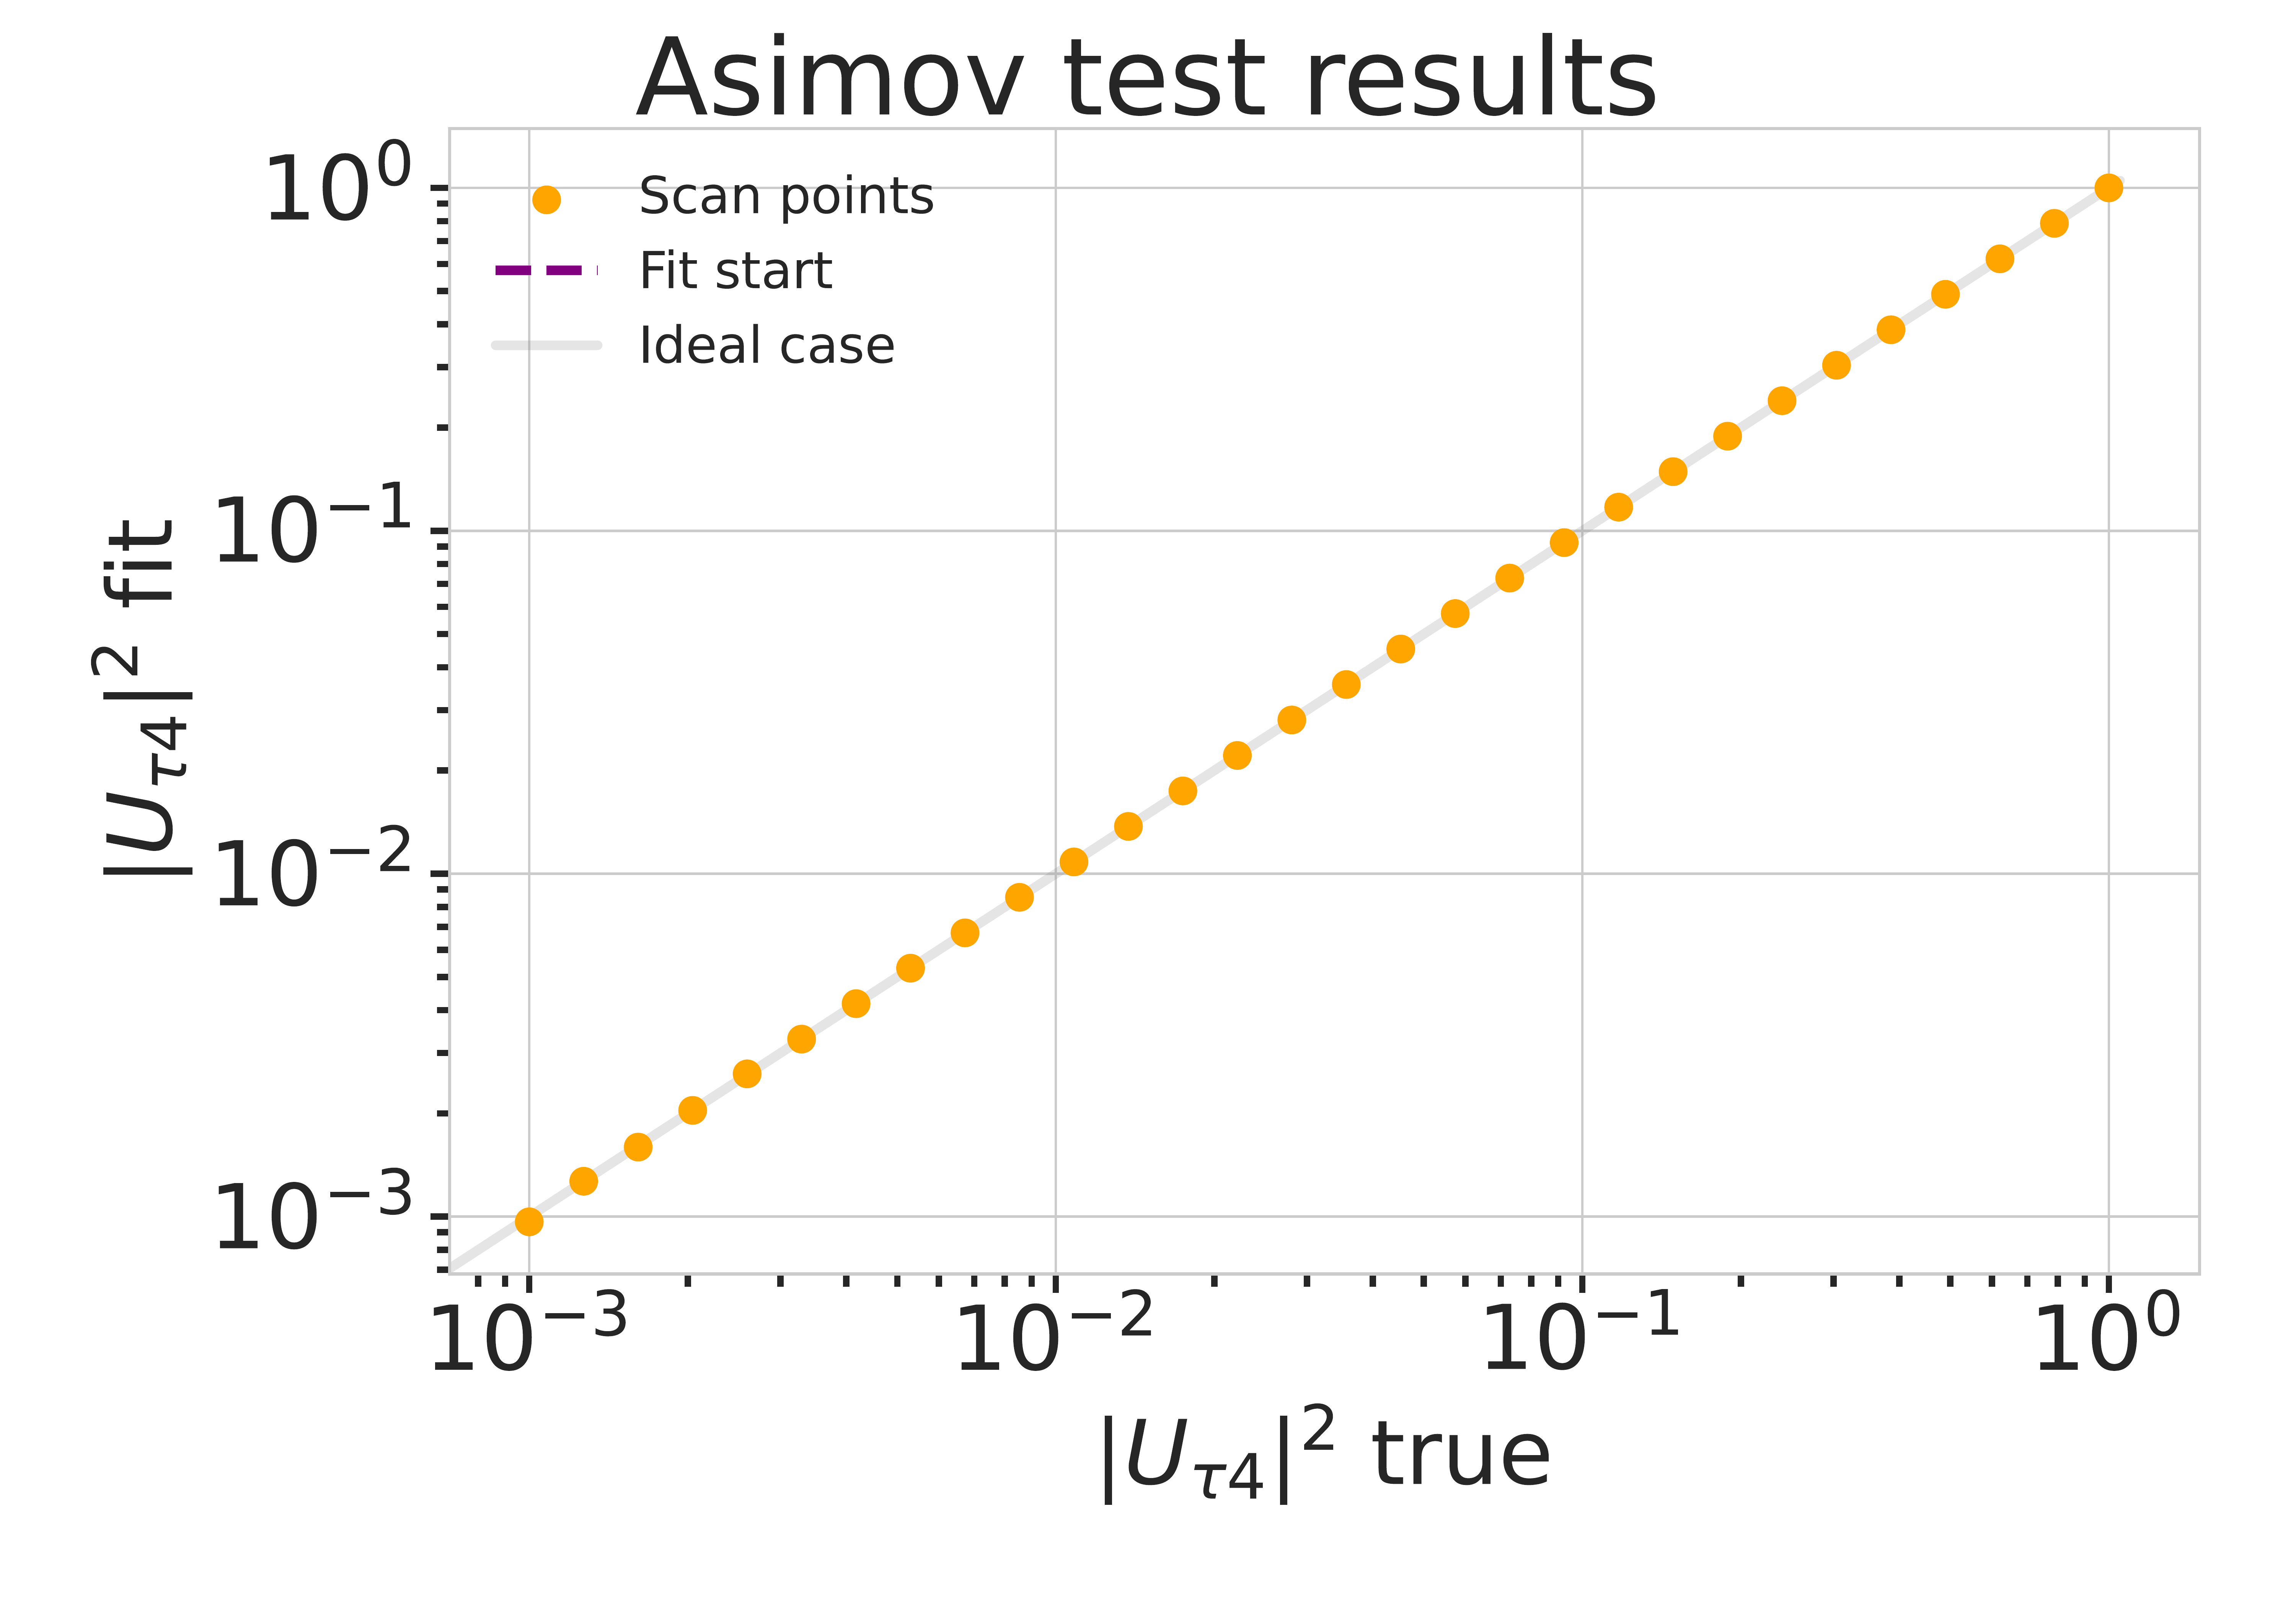
\includegraphics{figures/results/checks/asimov_scan_0.6_GeV-01.png}
	\caption[Asimov inject/recover test (\SI{0.6}{\gev})]{Asimov inject/recover test for the \SI{0.6}{\gev} mass set. Mixing values between $10^{-3}$ and $10^{0}$ are injected and fit back with the full analysis chain. The injected parameter is always recovered within the statistical uncertainty.}
    \labfig{asimov_inject_recover_0.6_GeV}
\end{figure}


% \subsection{Sensitivity}

% \begin{figure}[h]
%     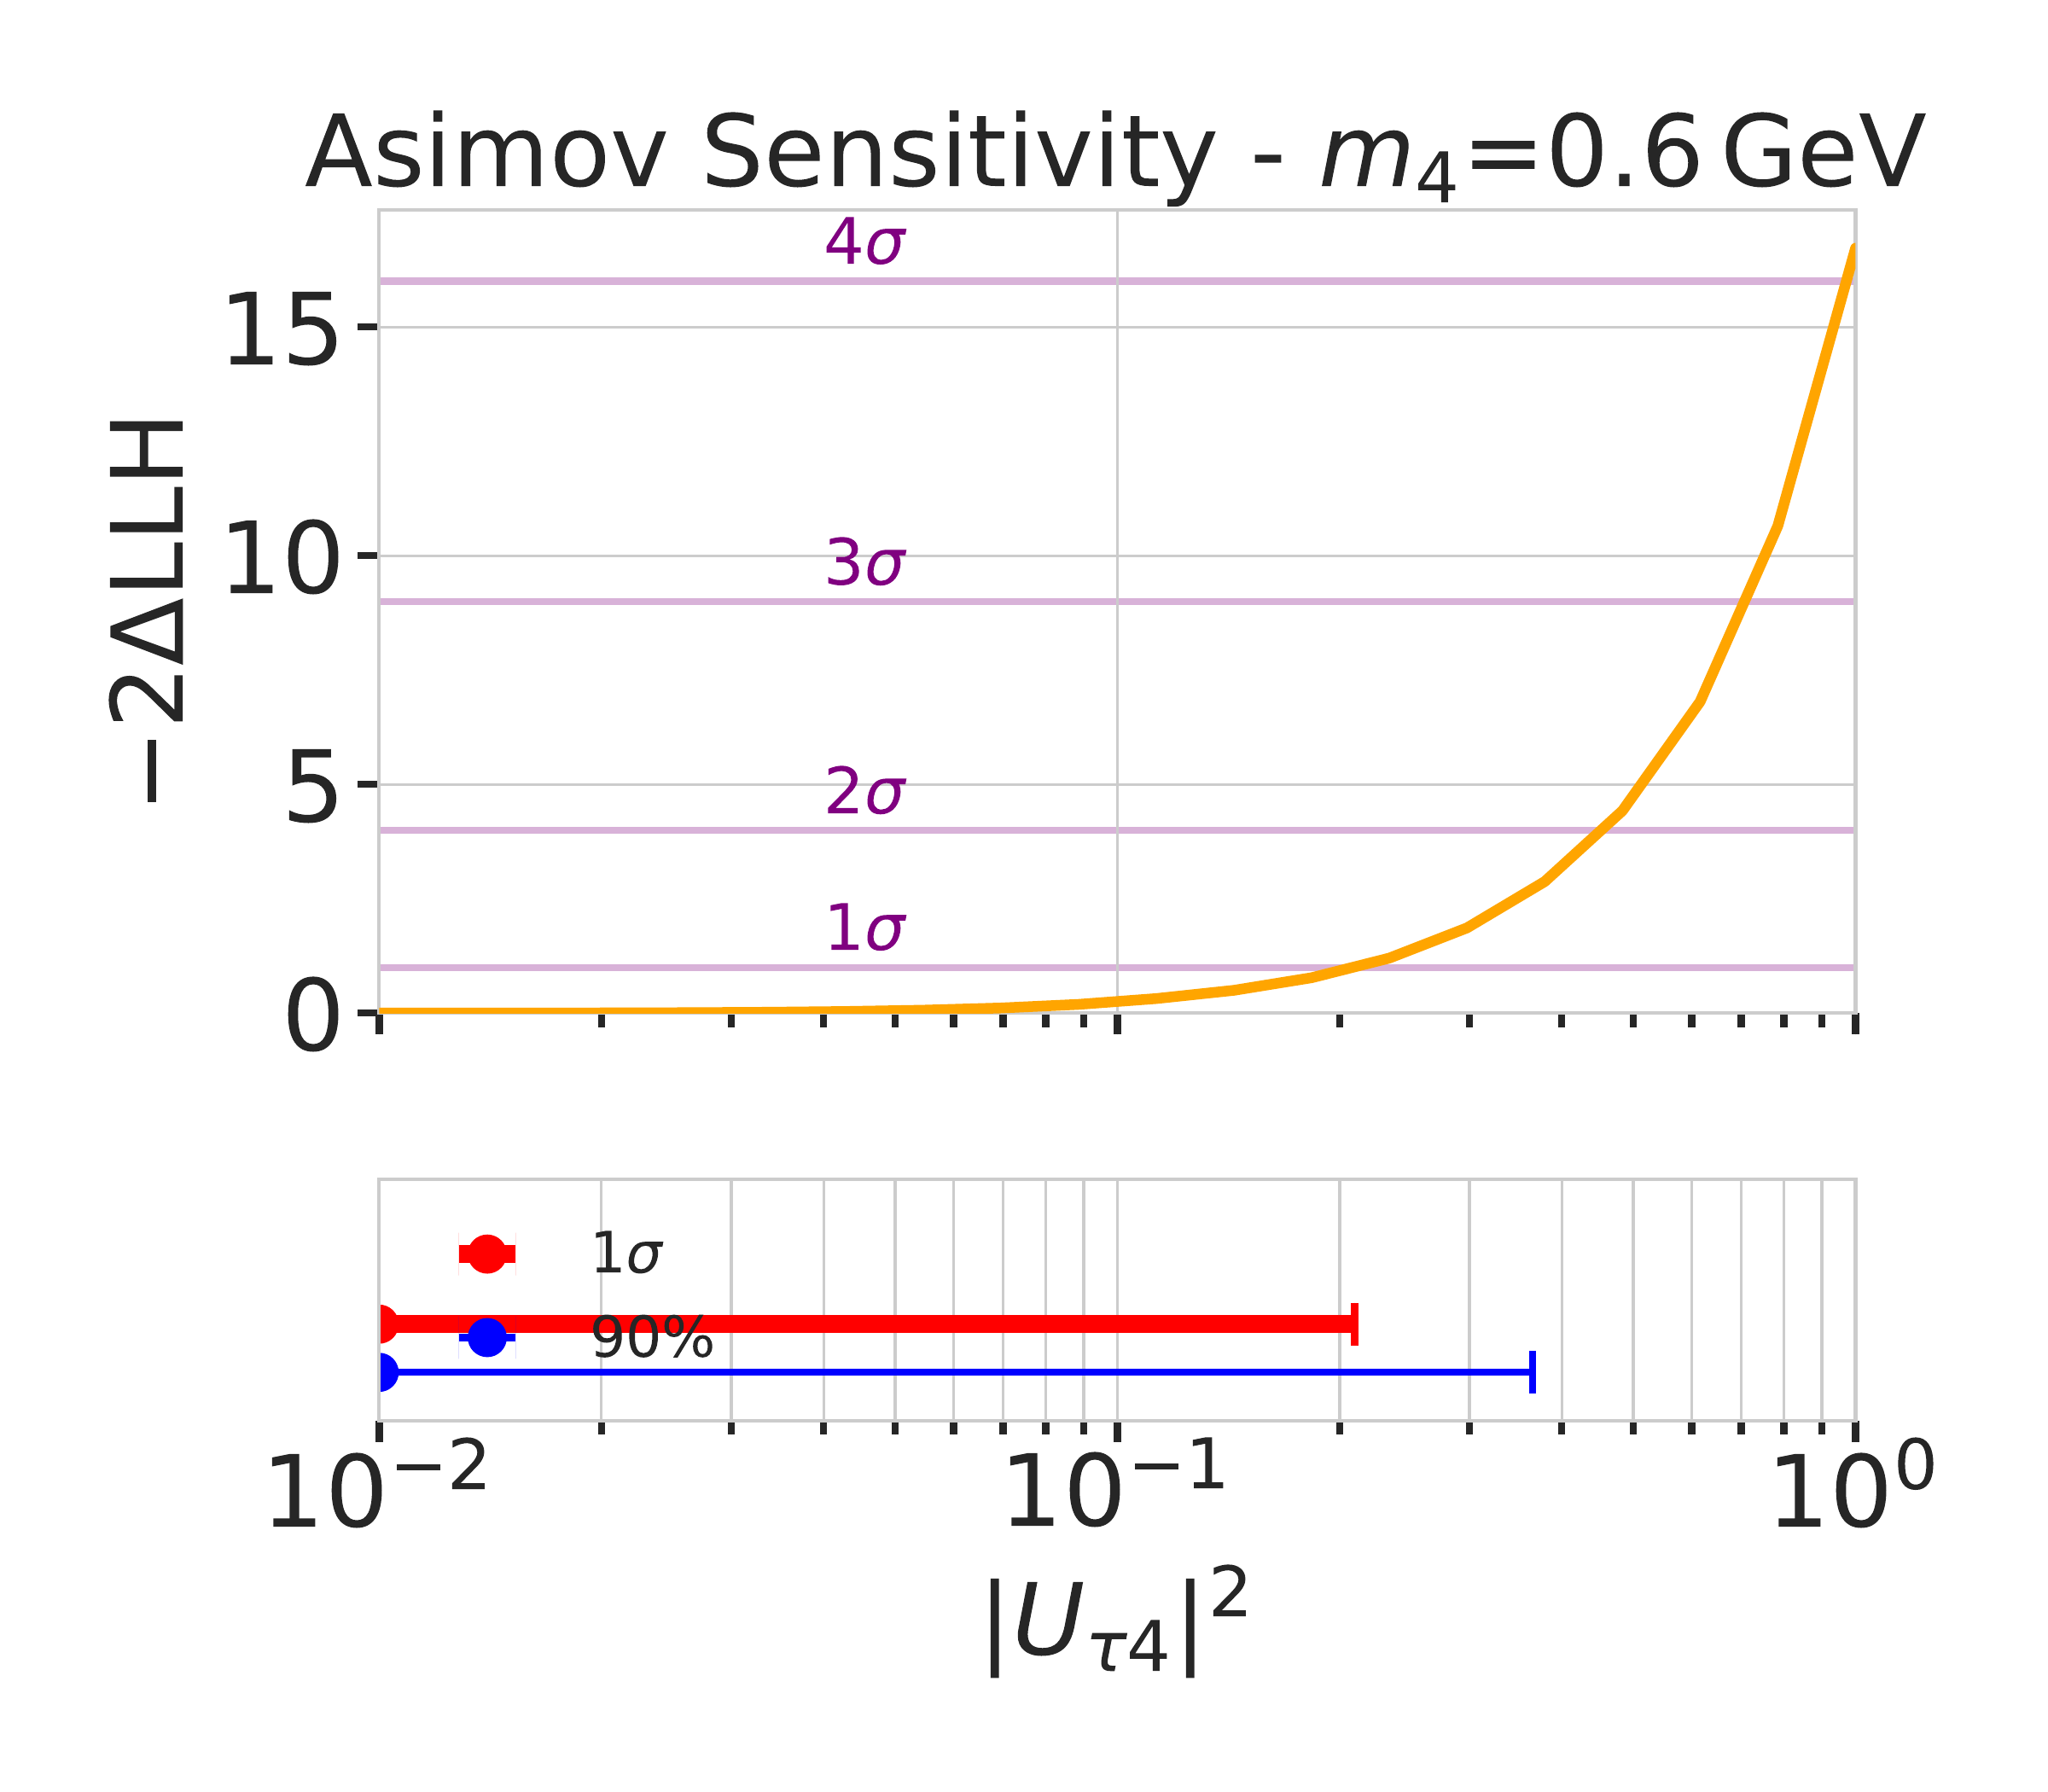
\includegraphics{figures/results/checks/sensitivity_scan_0.6_GeV-1.png}
% 	\caption[Sensitivity scan (\SI{0.6}{\gev})]{Sensitivity scan for the \SI{0.6}{\gev} mass set.}
%     \labfig{sensitivity_scan_0.6_GeV}
% \end{figure}


\subsection{Ensemble Tests} \labsec{pseudo_data_ensemble}

To estimate the goodness of fit, pseudo-data is generated from the MC by injecting the BFP parameters as true parameters and then fluctuating the expected bin counts to account for MC uncertainty and Poisson fluctuations in data. First, the expectation value of each bin is drawn from a Gaussian distribution centered at the nominal expectation value with a standard deviation corresponding to the MC uncertainty of the bin. Based on this sampled expectation value, each bin count is drawn from a Poisson distribution, independently, to get the final pseudo-data set. These pseudo-data sets are then fit back with the analysis chain. By comparing the distribution of TS values from this \textit{ensemble} of pseudo-data trials to the TS of the fit to real data, a p-value can be calculated. The p-value is the probability of finding a TS value at least as large as the one from the data fit. \reffig{pseudo_data_ensemble_0.6_GeV}\todo{Add bin-wise TS distribution? Add 3D TS maps?} shows the TS distribution from the ensemble tests for the \SI{0.6}{\gev} mass set and the observed TS value from the fit, resulting in a p-value of \SI{28.5}{\percent}. The p-values for the \SI{0.3}{\gev} and \SI{1.0}{\gev} are \SI{28.3}{\percent} and \SI{26.0}{\percent}, respectively and the correspoinding plots are shown in \refsec{pseudo_data_ensemble_appendix}.

% \sidenote{The p-values for the \SI{0.3}{\gev} and \SI{1.0}{\gev} are \SI{28.3}{\percent} and \SI{26.0}{\percent}, respectively.}
% 
\begin{figure}[h]
    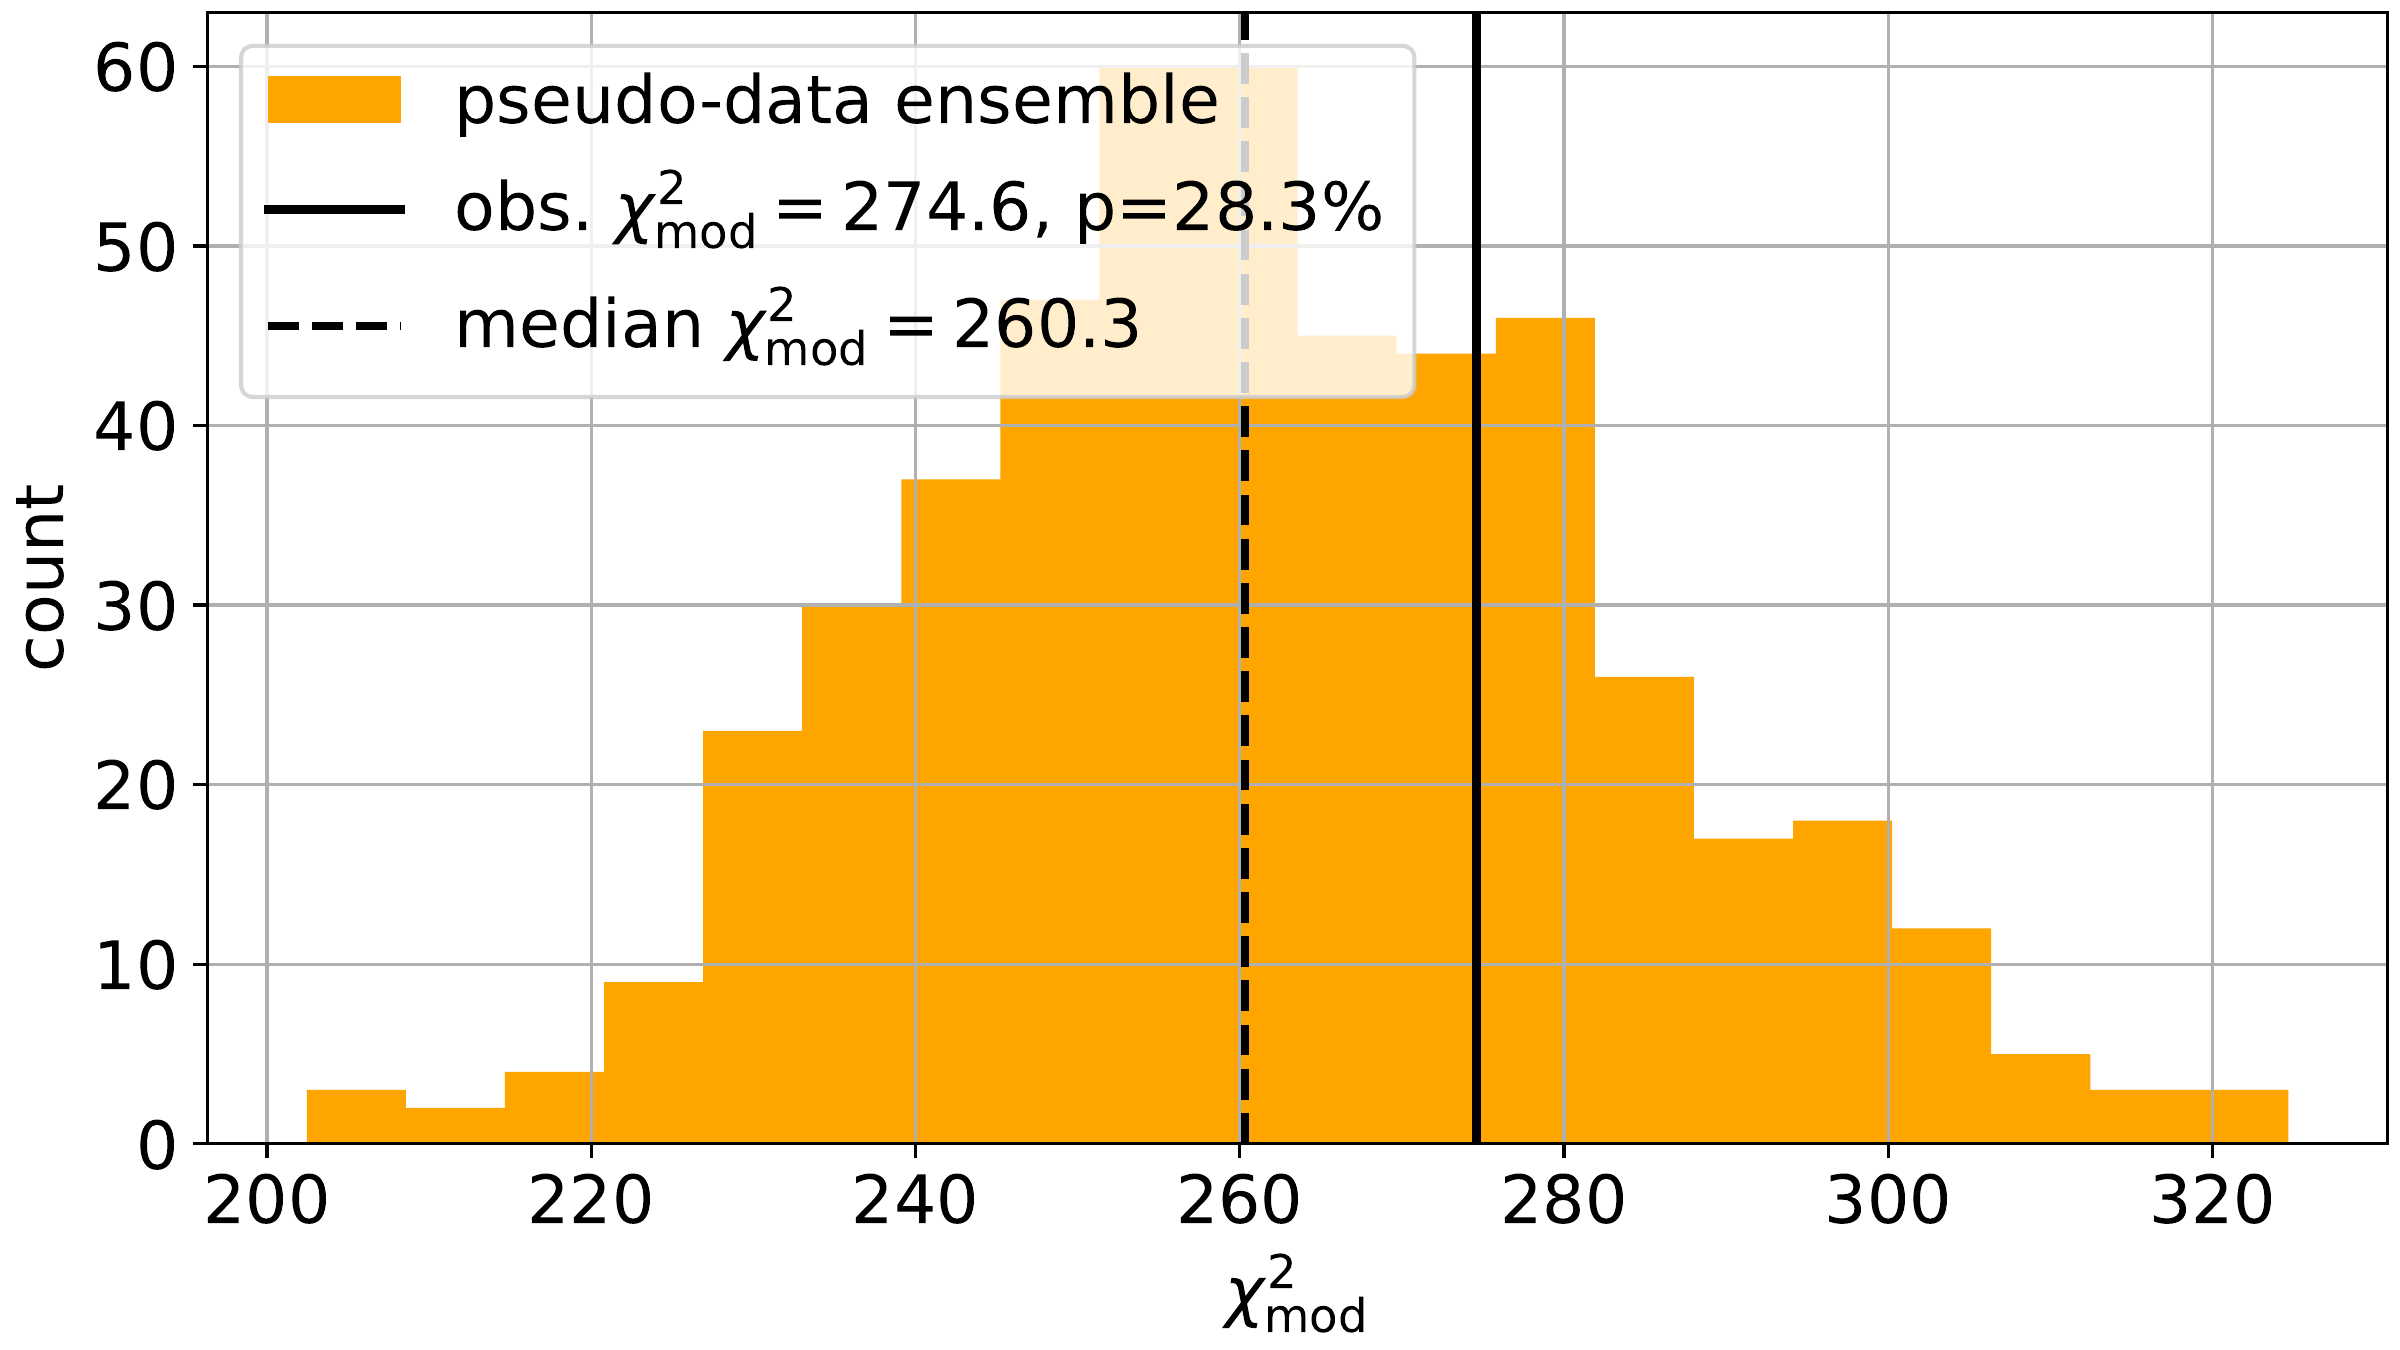
\includegraphics{figures/results/blind_fits/full_blind_fit_0.3_GeV_gauss_plus_poisson_step_3_4-1.png}
	\caption[Pseudo-data trials TS distribution (\SI{0.6}{\gev})]{Observed fit TS and TS distribution from pseudo-data trials for the \SI{0.6}{\gev} mass set.}
    \labfig{pseudo_data_ensemble_0.6_GeV}
\end{figure}


\section{Results}


\subsection{Best Fit Nuisance Parameters}

The resulting nuisance parameter values from the fits are illustrated in \reffig{best_fit_deltas_normed}, where the differences to the nominal values are shown, normalized by the distance to the closest boundary. The results from all three fits are shown in the same plot and the fits prefer values of the same size for all three mass sets. For parameters that had a Gaussian prior, the \SI{1}{\sigma} range is also displayed. As was already confirmed during the blind fit procedure, all fitted parameters are within this range, but the $\rm{Barr} \; h_{\pi^+}$ parameter is smaller and the $\rm{Barr} \; i_{\pi^+}$ is larger than expected, both being very close within the $+$\SI{1}{\sigma} and the $-$\SI{1}{\sigma} range, respectively. The $\rm{DIS}$ parameter fits to a smaller value than the nominal and all ice parameters, both $\rm{hole \, ice} \; p_0$, and $p_1$ as well as $\rm{bulk \, ice \, absorption}$, and $\rm{scattering}$ are found at values lower than the nominal. The effective ice model parameter, $N_\rm{bfr}$, prefers a value of $\sim$\SI{0.74}, indicating that the data is more \textit{BFR}-like (value of \SI{1.0}) than \textit{Spice 3.2.1}-like (value of \SI{0.0}). For completeness's sake, the explicit results are listed in \reftab{best_fit_parameters}. There, the nominal values and the absolute differences to the best fit value are also presented.

\begin{figure*}[h]
    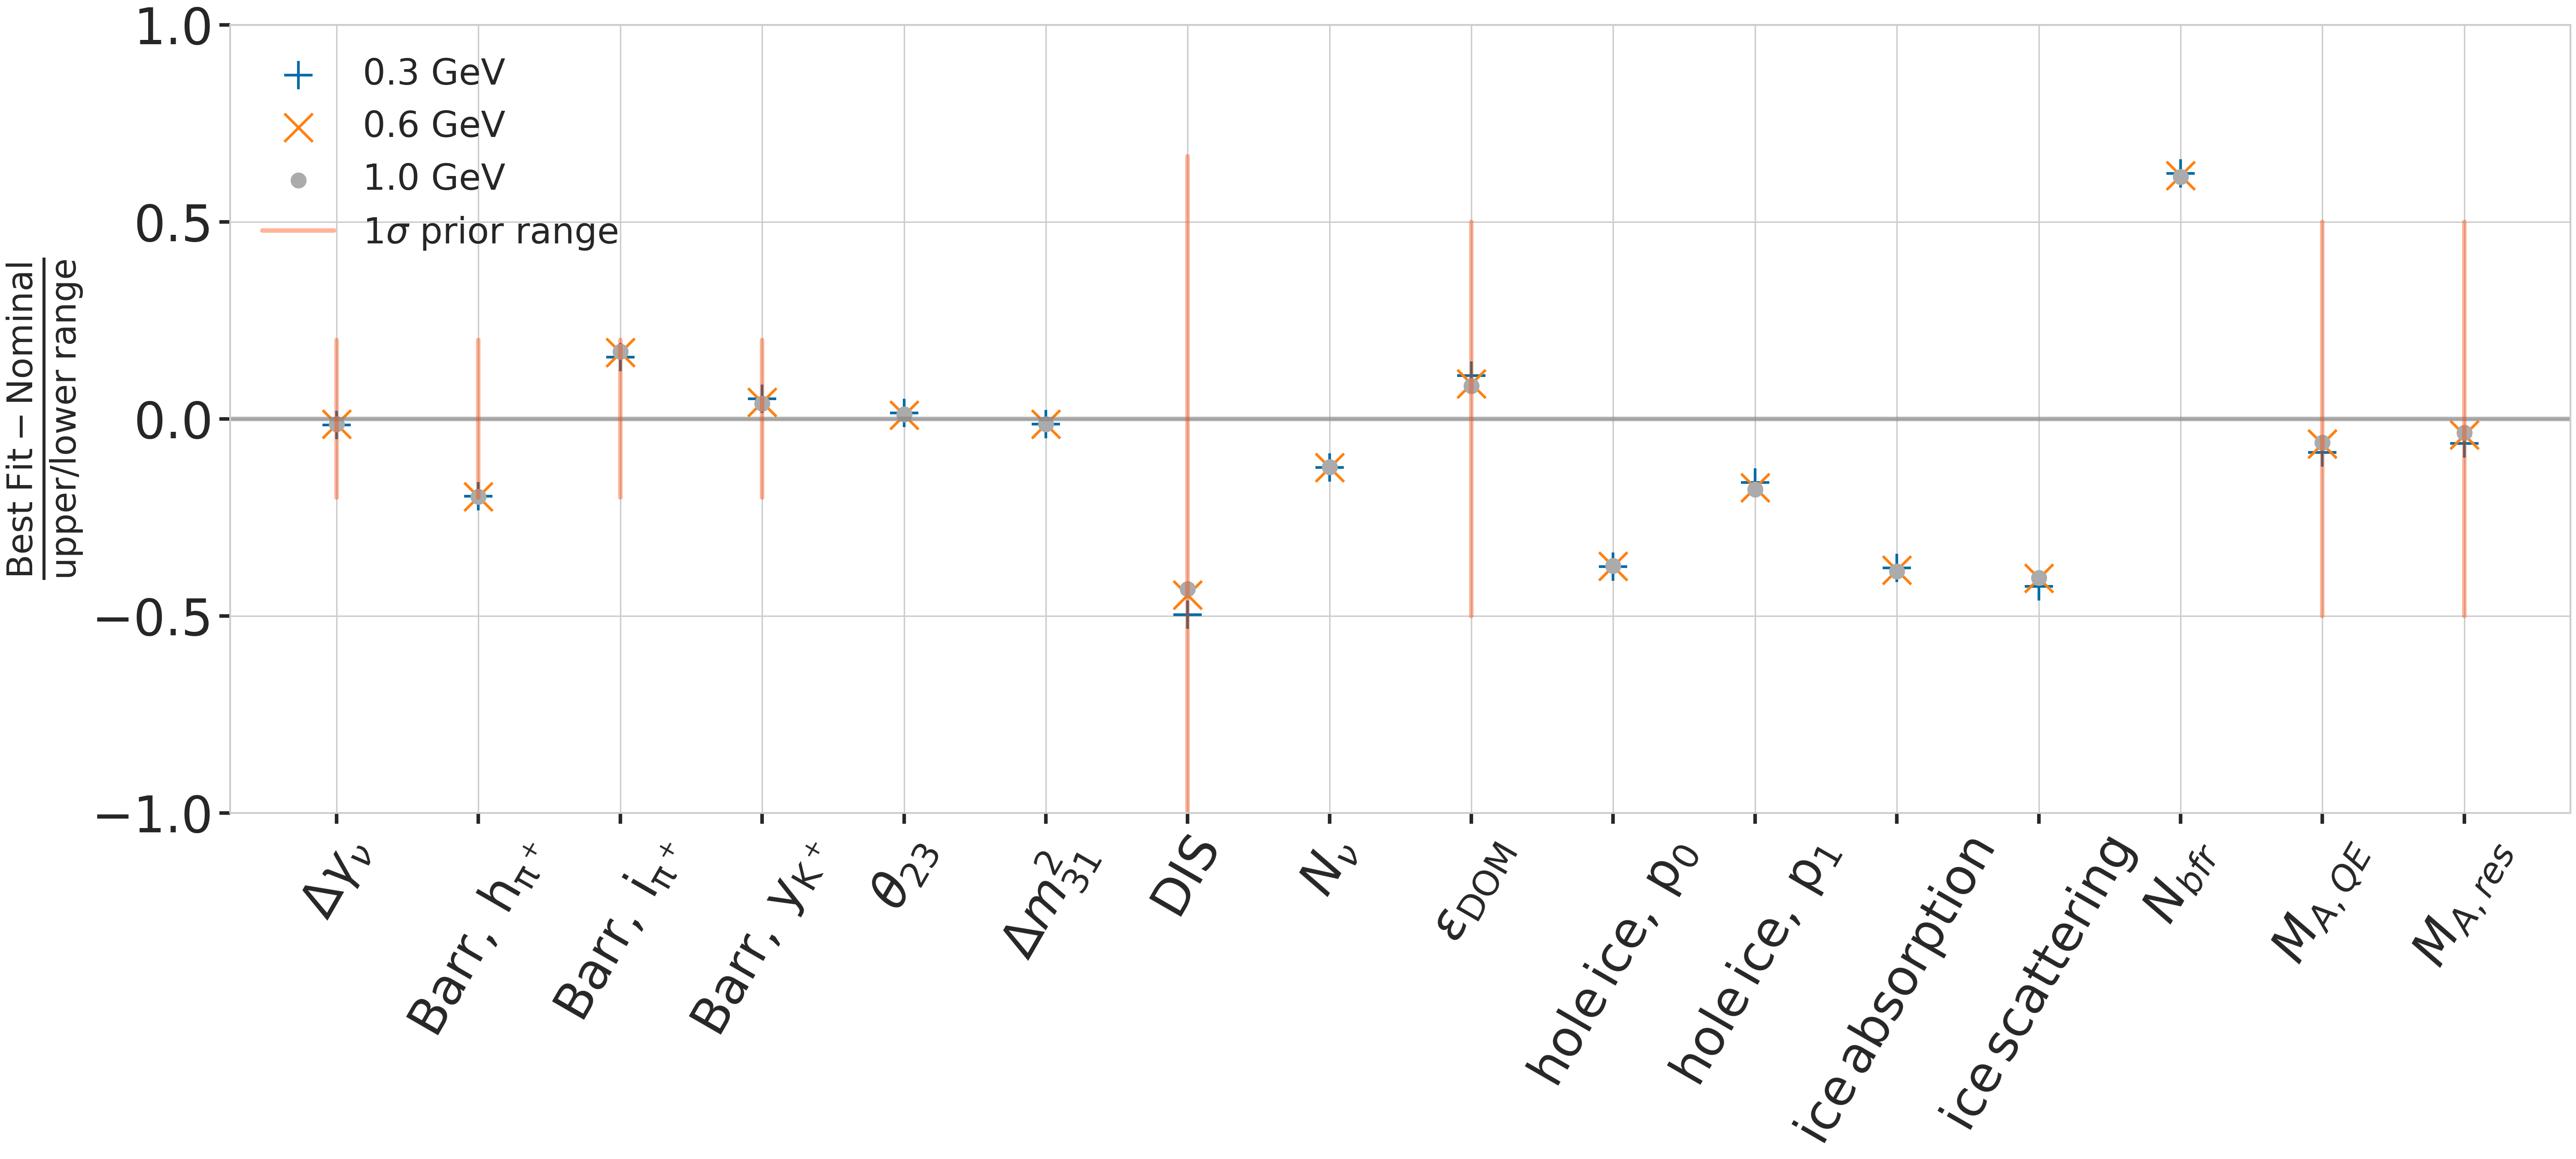
\includegraphics{figures/results/best_fit/hnl_analysis_best_fit_deltas_normed_dist_to_nominal_correct_0.6_fit.png}
	\caption[xx]{xx}
    \labfig{best_fit_deltas_normed}
\end{figure*}
\todo{fix caption for this figure}
\todo{sort the variables also by type, same as in the table "best\_fit\_parameters"?}

\todo{Show best fit hole ice angular acceptance compared to nominal and flasher/in-situ fits, maybe?}
\todo{Discuss what it means that the parameters are at these values? Here, or somewhere else?}


\subsection{Best Fit Parameters and Limits}

The fitted mixing values are
\begin{align*}
    |U_{\tau4}|^2_\rm{BFP}(\SI{0.3}{\gev}) &= 0.003^{+0.084} \;, \\
    |U_{\tau4}|^2_\rm{BFP}(\SI{0.6}{\gev}) &= 0.080^{+0.134} \;, \rm{and} \\
    |U_{\tau4}|^2_\rm{BFP}(\SI{1.0}{\gev}) &= 0.106^{+0.132} \;,
\end{align*}
with their $+$\SI{1}{\sigma} uncertainty. All of them are compatible with the null hypothesis of \SI{0.0} mixing, although the \SI{0.6}{\gev} and \SI{1.0}{\gev} fits indicate a mixing value around \SI{0.09}. The best fit mixing values and the corresponding upper limits at \SI{68}{\percent} and \SI{90}{\percent} \textit{confidence level (CL)} are listed in \reftab{best_fit_parameters_and_confidence_levels}, also showing the CL at the null hypothesis, which is the probability of excluding the null hypothesis with this fit. The CLs are estimated by assuming that \textit{Wilks' theorem} \sidecite{the_not_to_be_mentioned_theorem} holds, meaning that the TS follows a $\chi^2$ distribution with one degree of freedom.

\begin{table}[h]
    % \footnotesize
    
    \begin{tabular}{ lllll }
        \hline\hline
    
        \textbf{HNL mass} & \textbf{$|U_{\tau4}|^2_\rm{BFP}$} & \textbf{68 \si{\percent} CL} & \textbf{90 \si{\percent} CL} & \textbf{CL$_\rm{null\,hypo}$} \\
        % \textbf{$m_4$ [\si{\gev}]} & \textbf{$|U_{\tau4}|^2_\rm{BFP}$} & \textbf{68 \si{\percent} CL} & \textbf{90 \si{\percent} CL} & \textbf{$\Delta\chi^2_{\mathrm{mod,null}}$} \\
    
        \hline\hline

        \SI{0.3}{\gev} & 0.003 & 0.087 & 0.194 & \SI{0.03}{\percent} \\
        \SI{0.6}{\gev} & 0.080 & 0.214 & 0.355 & \SI{21.29}{\percent} \\
        \SI{1.0}{\gev} & 0.106 & 0.238 & 0.396 & \SI{37.25}{\percent} \\
        \hline
    \end{tabular}

    % % didn't work in the margin..
    % \begin{tabular}{ llll }
    %     \hline\hline
    
    %     % \textbf{HNL mass} & \textbf{\SI{0.3}{\gev}} & \textbf{\SI{0.6}{\gev}} & \textbf{\SI{1.0}{\gev}} \\
    %     \textbf{$m_4$ [\si{\gev}]} & \textbf{\SI{0.3}{}} & \textbf{\SI{0.6}{}} & \textbf{\SI{1.0}{}} \\
    
    %     \hline\hline

    %     \textbf{$|U_{\tau4}|^2_\rm{BFP}$} & 0.003 & 0.080 & 0.106 \\
    %     \textbf{68 \si{\percent} CL} & 0.087 & 0.214 & 0.238 \\
    %     \textbf{90 \si{\percent} CL} & 0.194 & 0.355 & 0.396 \\
    %     \hline
    %     \textbf{CL$_\rm{null}$ [\si{\percent}]} & \SI{0.03}{} & \SI{21.29}{} & \SI{37.25}{} \\
    %     \hline
    % \end{tabular}

    \caption[xx]{xx}
    \labtab{best_fit_parameters_and_confidence_levels}
\end{table}
\todo{fix table caption}

\reffig{brazil_band_0.6_GeV} shows the observed likelihood profile for the \SI{0.6}{\gev}, which is the difference in $\chi^2_{\mathrm{mod}}$ between the best fit and each scan point in $|U_{\tau4}|^2$. Also shown is the expected likelihood profile, based on a scan over Asimov data, also produced at the BFP. The observed CLs are slightly larger/smaller\todo{fix once I have them produced} than the expected CL. To ensure this is compatible with random fluctuations, the expected likelihood is also profiled for 100 pseudo-data sets, which are generated at the BFP and then fluctuated using both Poisson and Gaussian fluctuations, to include the data and the MC uncertainty, as was already done for the ensemble tests. The resulting CLs are shown as the colored areas and the observed contour is well within the \SI{68}{\percent} band, confirming that it is compatible with data fluctuations. \reffig{brazil_bands_appendix} shows the same likelihood profiles and bands for the other two mass sets. For both of them the observed CLs are also slightly larger/smaller than the expected, but still within the \SI{68}{\percent} band of the pseudo-data trials, so they are also compatible with random fluctuations.

\begin{figure}[h]
    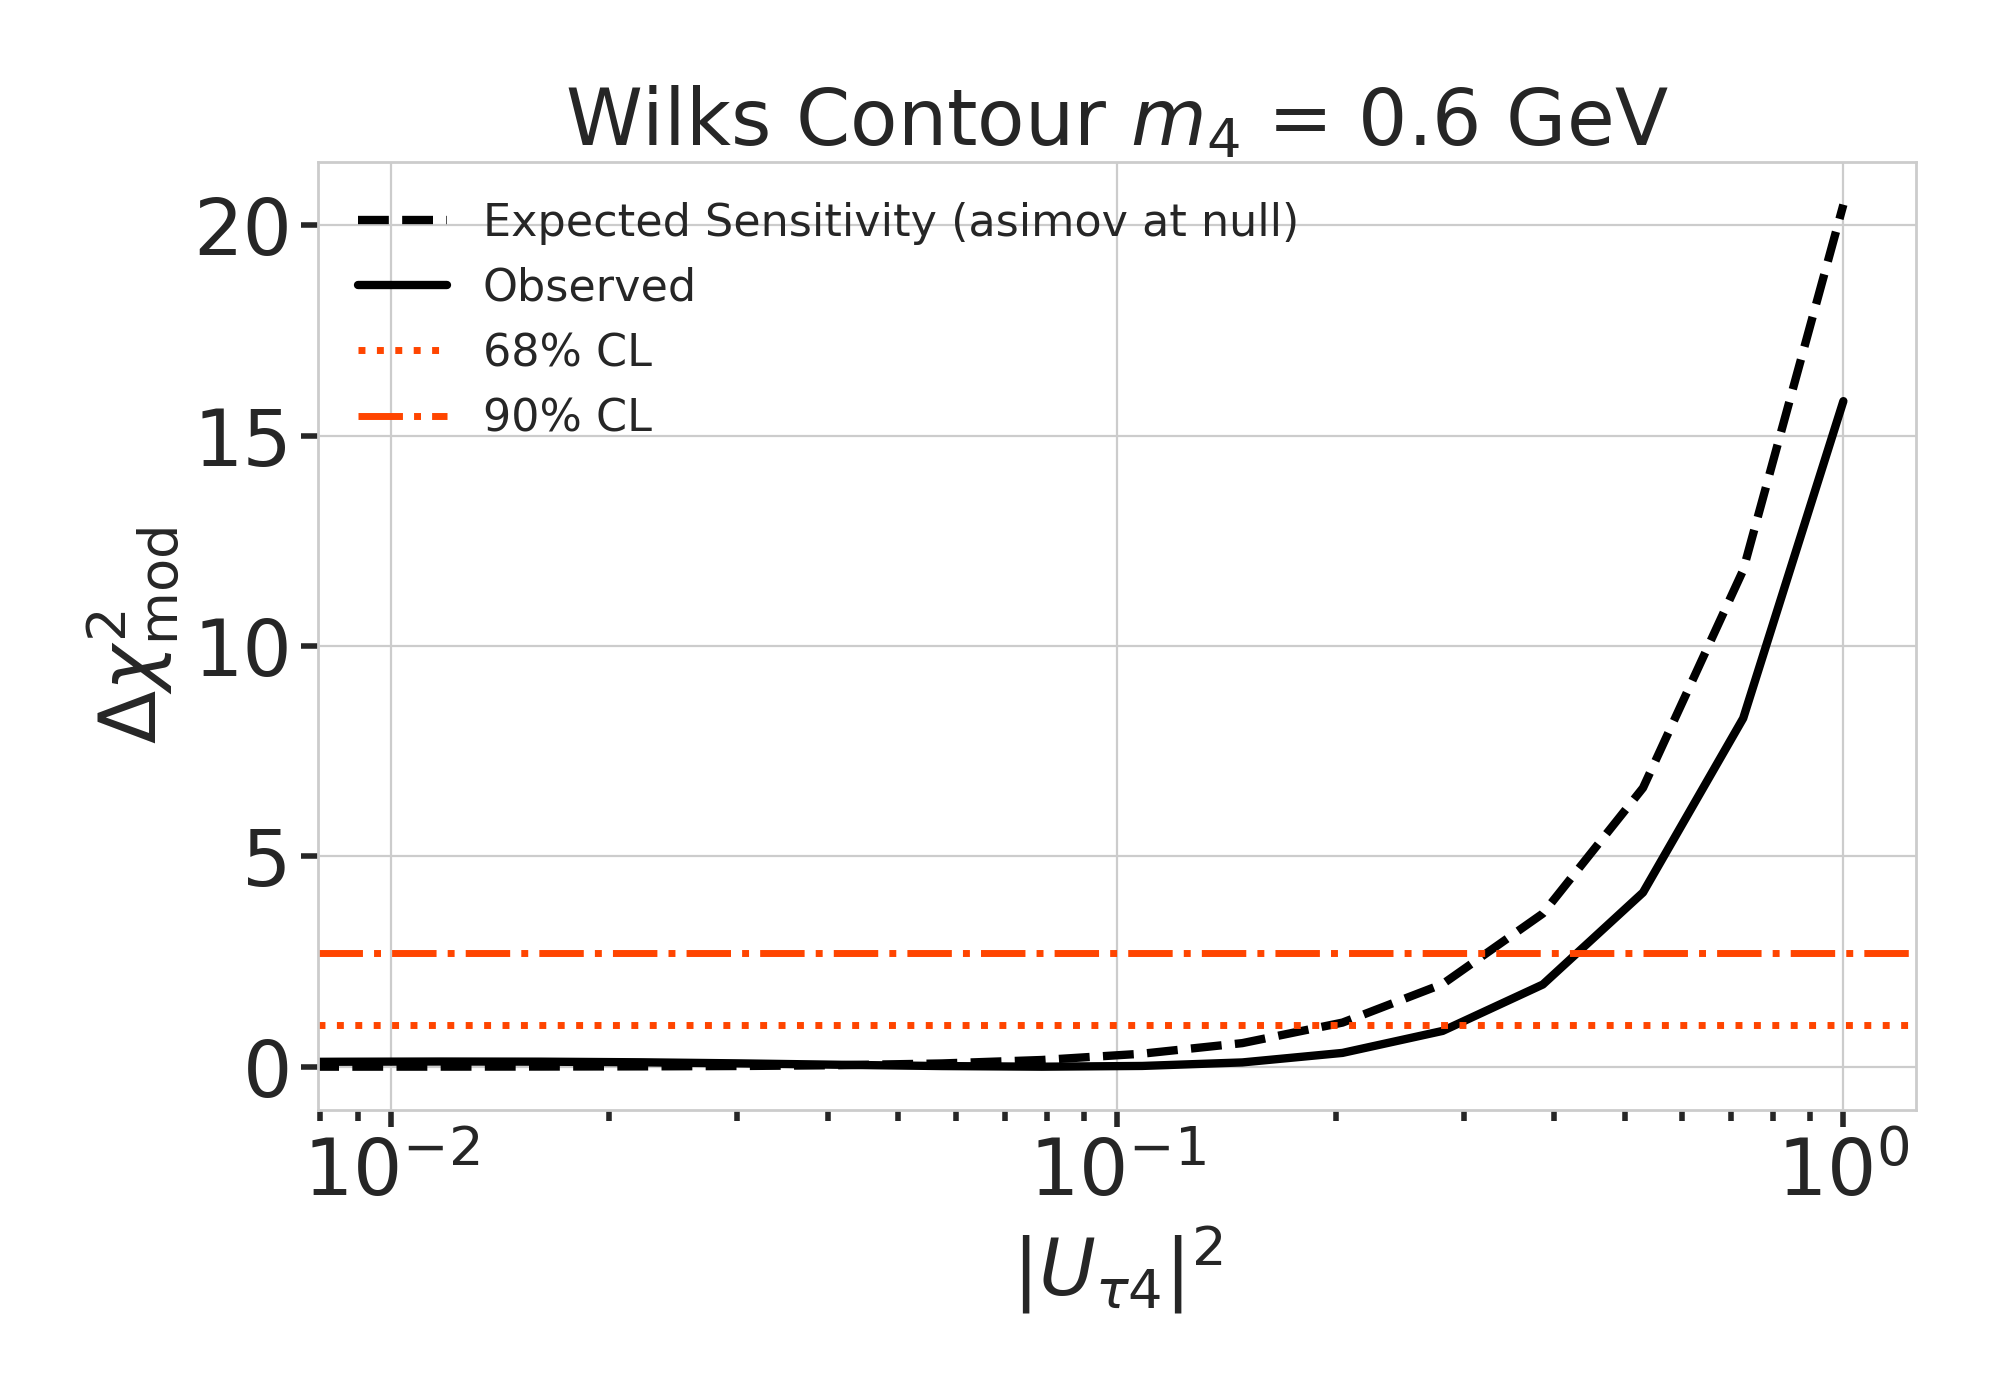
\includegraphics{figures/results/best_fit/sensitivity_and_wilks_scan_0.6_GeV_with_1sigma.png}
	\caption[xx]{xx}
    \labfig{brazil_band_0.6_GeV}
\end{figure}
\todo{fix caption for this figure}

% \begin{figure}[h]
%     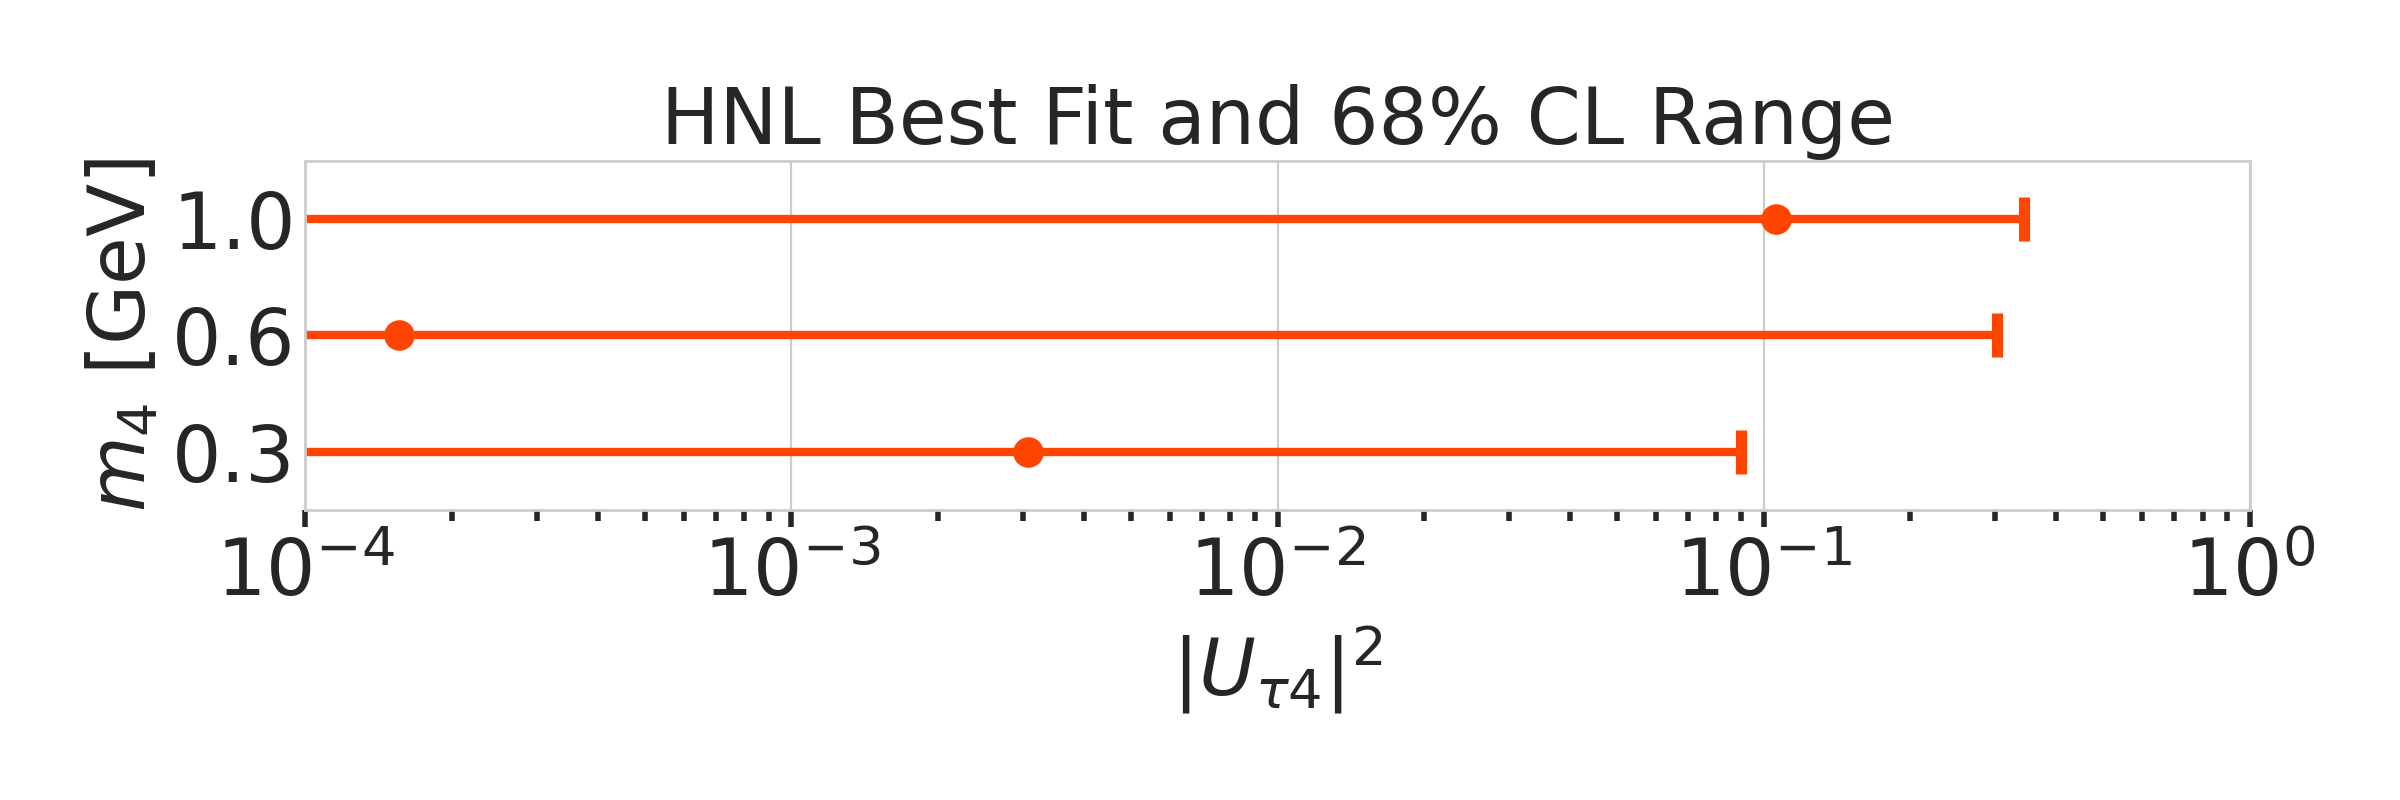
\includegraphics{figures/results/best_fit/best_fit_results_and_limits.png}
% 	\caption[xx]{xx}
%     \labfig{best_fit_mixings_and_limit}
% \end{figure}
% \todo{fix caption for this figure}

\todo{make plot with BFPs and limit, comparing to upper limits from other experiments}


\subsection{Data/MC Agreement}

At the BFP, the agreement between the data and simulation is probed by comparing the 1-dimensional analysis distributions for PID, energy, and cosine of the zenith angle. As an example, two distributions\todo{specify which they are, once I have them} for the \SI{0.6}{\gev} mass set are shown in \reffig{data_mc_agreement_0.6_GeV}. The data is compared to the total MC expectation, which is also split up into its composing parts. Good agreement can be observed in the pull distributions and is quantified by a reduced $\chi^2$, which is close to \SI{1.0} for all distributions. The reduced $\chi^2$ for all investigated distributions is listed in \reftab{data_mc_agreement}, while the distributions themselves can be found in \refsec{data_mc_agreement_appendix}.

\todo{add 1-d data/mc agreement for example mass set (0.6?) and all 3 analysis variables}
\todo{add table with reduced chi2 for all 1-d distributions}

\subsection{Likelihood Coverage}

To find the CLs, the profile likelihood was evaluated by applying Wilks' theorem. It isn't guaranteed however, that the theorem holds and it is therefore important to check the \textit{coverage} of the likelihood. 
